%% This document shows an example of writing exam paper in a single file.
%% tailored for PPK Alam sekitar, ppkas
%%
\documentclass[12pt]{article}
%% Enable either one of these %%
%\usepackage{finalxm}			% standard for everyone
%\usepackage[ppkas,ftquestionnum]{finalxm}			% Figure 1.1
\usepackage[ppkas,ftquestionnumx]{finalxm}			% Figure A1.1
%\usepackage[ppkas,ftquestionnum, minutes]{finalxm}		% show hours & minutes
%\usepackage[ppkas,ftquestionnumx, minutes]{finalxm}	% show hours & minutes
%\usepackage[ppkas,ftquestionnum, answers]{finalxm}	% answer scheme
%\usepackage[ppkas,ftquestionnumx, answers]{finalxm}	% answer scheme
%\usepackage{pdflscape}	% for landscape layout on specific page 
%
% Declare graphics path 
 \graphicspath{{./Figures/}}	% a subfolder named figs

%%%%%%%%%%%%%%%%%%%%%%%%%%%
%%% PERSONALIZED STYLES %%%
%%%%%%%%%%%%%%%%%%%%%%%%%%%

%% TABLE/FIGURE WITH CAPTION %%
%% Options availabe for caption. put these before begin{figure/table}
%% font, labelfont, textfont || use either bf, normalfont
%% labelsep || use either newline, colon
%\captionsetup[figure]{labelsep=newline, font=normalfont} 	% all bold
%\captionsetup[table]{labelsep=newline, font=normalfont}	% all bold
%\captionsetup[figure]{labelsep=colon} 	% all bold
%\captionsetup[table]{labelsep=colon}	% all bold
%\captionsetup[figure]{labelsep=colon, textfont=normalfont} 	% bold Figure
%\captionsetup[table]{labelsep=colon, textfont=normalfont} 	% bold Table
%\captionsetup[figure]{labelsep=colon, font=normalfont} 	% all no bold 
%\captionsetup[table]{labelsep=colon, font=normalfont} 	% all no bold 

%%%%%%%%%%%%%%%%%%%%%%%%
%%% SETUP TITLE PAGE %%%
%%%%%%%%%%%%%%%%%%%%%%%%
\mtefe{Pertengahan} 			% Akhir, Pertengahan 
\semester{Kedua}		% Pertama, Kedua
\sidang{2017/2018}		
\examMonthYear{27 Mac 2018}
\courseCode{ENT390}
\courseNameEn{Bioinstrumentation 1}
\courseNameBM{Bioinstrumentasi 1}
\pagesbm{TIGA PULUH SATU}	% used if the number of pages exceeds 30
\durationhr{1 Jam}		% duration of exam
\makeatletter 
\if@minutes
	\durationmin{30 Minit}	% MUST be enabled using \usepackage[minutes]{finalxm}
\fi 		
\makeatother		

\begin{document}
\makecover	% make cover/title page

\instructionen{
	This question paper has \textbf{TWO (2)} questions. Answer \textbf{all} questions. Each question contributes 25 marks.%
}
\instructionbm{%
	Kertas soalan ini mengandungi \textbf{DUA (2)} soalan. Jawab \textbf{semua} soalan. Setiap soalan menyumbang 25 markah.%
}

% Delete from here if require no extra notes 
\vskip 3em
\instructionen{
	Note: This is extra instructions%
}
\instructionbm{%
	Ini adalah arahan tambahan.%
}
% Delete until here if require no extra notes 

\makecoverend	% end cover/title page

%%%%%%%%%%%%%%%%%%%%%%%%%%%%
%%% MAIN BODY START HERE %%%
%%%%%%%%%%%%%%%%%%%%%%%%%%%%
\setmainstyle
\vskip -2em		% adjust vertical space skip accordingly 

%%%%%%%%%%%%%
%%% PART  %%%
%%%%%%%%%%%%%
%\textbf{Answer all questions} 
%
%\translationbf{Jawab semua soalan}
%\bigskip
\begin{framed}
	\newparten{}This section has \textbf{FOUR (4)} questions. Answer \textbf{ALL} questions.

	\newpartbmx{Bahagian ini mengandungi \textbf{EMPAT (4)} soalan. Jawab \textbf{SEMUA} soalan.}
\end{framed}


%%%%%%%%%%%%%%%%%%
%%% QUESTION 1 %%%
%%%%%%%%%%%%%%%%%%
%TODO Question1
\bigskip 
%\partQuestion{[CO1, PO1]}
\question{}[\label{q1label}]

\listbeginx	% start 1st level question
	\item \label{item:infusion} Infusion pumps are designed to assist in fluids delivery into a patient's body in controlled amounts. Force and pressure sensors are used to ensure the desired amount of fluid is being delivered to the patient and detect occlusion, if any. 
	
	\translation{Pam infusi direka bentuk untuk membantu dalam memasukkan cecair ke dalam badan pesakit dengan jumlah yang terkawal. Penderia daya dan tekanan digunakan untuk memastikan jumlah cecair yang dikehendaki dihantar dan mengesan sekatan, sekiranya ada.} 
	
	\listbegin
		\item \label{item:sensor} Suggest a suitable type of sensor to detect force and pressure changes, and justify your suggestion.
		
		\translation{Cadangkan jenis penderia yang sesuai untuk mengesan perubahan daya dan tekanan, dan wajarkan cadangan anda.}
		
		\qmarks{3}	% define marks
		
		\item Elaborate \textbf{TWO (2)} sensor characteristics that are deemed importance for infusion pump as described in Q\ref{q1label}\ref{item:infusion}\ref{item:sensor}
		
		\translation{Huraikan \textbf{DUA (2)} ciri-ciri penderia yang disifatkan penting untuk pam infusi.}
		
		\qmarks{4}

	\listclose % close 2nd level
	
	\item You are given a task to design a capacitive sensor that is able to pass sound frequencies above 25 Hz. For a 1.5 $cm^2$ capacitance sensor, $R$ is 10~\si{\mega\ohm}. (Relative Permitivity $= 8.8854 \times~10^{-12}$)
	
	\translation{Anda diberikan tugasan untuk mereka bentuk penderia kapasitan yang mampu membenarkan frekuensi bunyi lebih 25~Hz. Untuk 1.5~$cm^2$ penderia kapasitan, R adalah \emph{10~\si{\mega\ohm}}. Ketelusan relatif $= 8.854 \times 10^{-12}$,}
	
	\begin{figure}[H] % H means, to put figure here after the code
		\centering
		%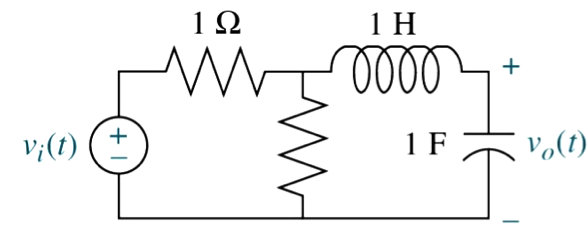
\includegraphics[width=0.5\textwidth]{testfig}
		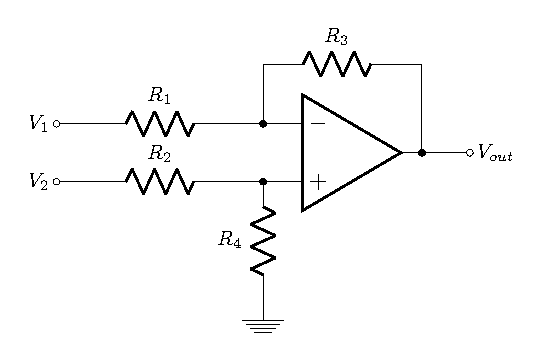
\includegraphics{diffamp}
%		\caption{Differential Amplifier \\ \figurecaption{Penguat Pembeza}}
		\caption{\rajah}
		\label{fig:diffamp}
	\end{figure}
	
\listclose % close 1st level question

%\nextpage % put the ...page/-
%\clearpage	% end question and start new page


%%%%%%%%%%%%%%%%%%
%%% QUESTION 2 %%%
%%%%%%%%%%%%%%%%%%
%TODO Question2
\clearpage		% page break
\question{}
%\partQuestion{}

\listbeginx	% start 1st level question
	\item Bioelectric potentials are produced as a result of electrochemical activity of an excitable cell. In resting state where there is no stimulus, the cell is polarized.
	
	\translation{Daya bioelektrik dihasilkan dari kesan aktiviti elektrokimia sesuatu sel peka rangsang. Dalam keadaan rehat di mana tiada rangsangan, sel adalah terkutub.}
	
	\listbegin
		\item What is the typical value of cell membrane potential in resting state, and how it is measured?
		
		\translation{Apakah nilai daya membran sel dalam keadaan rehat, dan bagaimana ianya diukur?}
		
		\qmarks{2}
		
		\item Elaborate how the cell membrane potential maintained polarized in resting state.
		
		\translation{Huraikan bagaimana daya membran sel kekal terkutub sewaktu keadaan rehat.}
		
		\qmarks{8}
		
		\item Differentiate between absolute refractory period and relative refractory period, and why the value differs in ventricular cell?
		
		\translation{Bezakan di antara tempoh refraktori mutlak dan tempoh refraktori relatif, dan kenapa nilai ini berbeza untuk sel ventrikular?}
		
		\qmarks{5}
	\listclose 
	
%	\nextpage 
%	\clearpage 
	
	\item The simplest configuration of instrumentation amplifier (INA) is shown in \cref{fig:diffamp}. 
	
	\translation{Tatarajah paling mudah bagi penguat instrumentasi (INA) ditunjukkan dalam \Cref{fig:diffamp}.}
	
%	\captionsetup[figure]{labelsep=newline, font=normalfont} 	% all bold
	\begin{figure}[H] % H means, to put figure here after the code		
		\centering
		%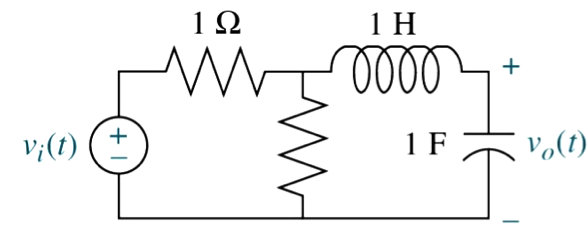
\includegraphics[width=0.5\textwidth]{testfig}
		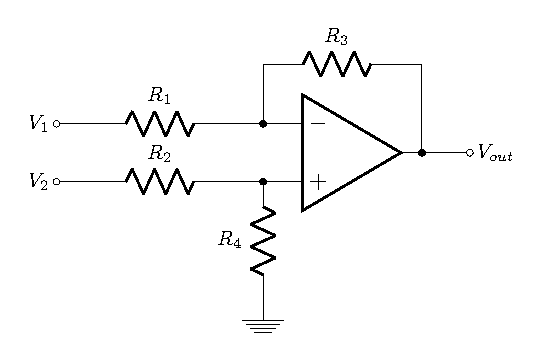
\includegraphics{diffamp}
%		\caption{Differential Amplifier \\ \figurecaption{Penguat Pembeza}}
		\caption{\rajah}
		\label{fig:diffamp2}
	\end{figure}

%	\captionsetup[figure]{labelsep=newline, font=bf} 	% all bold
	\begin{figure}[H] % H means, to put figure here after the code		
		\centering
		%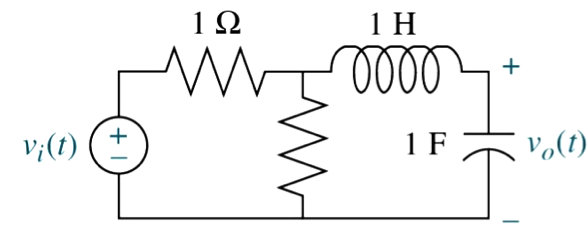
\includegraphics[width=0.5\textwidth]{testfig}
		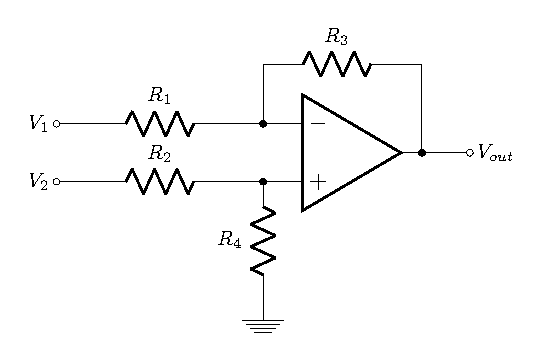
\includegraphics{diffamp}
		%	\caption{Differential Amplifier \\ \figurecaption{Penguat Pembeza}}
		\caption{\rajah}
		\label{fig:diffamp3}
	\end{figure}
	
%	\captionsetup[table]{labelsep=colon}	% all bold
	% Table generated by Excel2LaTeX from sheet 'Sheet1'
	\begin{table}[H]
		\centering
		\caption{Freq. vs Magnitude \\ \tablecaption{Frekuensi vs Magnitud}}
%		\caption{\jadual}	% no caption
		%		\begin{tabularx}{220pt}{c c}
		\begin{tabular}{cc}
			\toprule
			% \toprule[1.5pt]
			\multicolumn{1}{l}{\textbf{Frequency}} & \multicolumn{1}{l}{\textbf{Impedance (Magnitude) ($\Omega$)}} \\
			\midrule
			5 Hz  & 20,000 \\
			10 Hz & 19,998 \\
			\vdots     & \vdots \\
			40 kHz & 602 \\
			50 kHz & 600 \\
			100 kHz & 600 \\
			\bottomrule
			%			\bottomrule[1.5pt]
		\end{tabular}
		%		\end{tabularx}%
		\label{table:freqmag}%
	\end{table}%
	
	\captionsetup[table]{labelsep=newline, font=normalfont}	% no bold
	% Table generated by Excel2LaTeX from sheet 'Sheet1'
	\begin{table}[H]
		\centering
%		\caption{Freq. vs Magnitude \\ \tablecaption{Frekuensi vs Magnitud}}
		\caption{\jadual}	% no caption
		%\begin{tabularx}{220pt}{c c}
		\begin{tabular}{cc}
			\toprule
			% \toprule[1.5pt]
			\multicolumn{1}{l}{\textbf{Frequency}} & \multicolumn{1}{l}{\textbf{Impedance (Magnitude) ($\Omega$)}} \\
			\midrule
			5 Hz  & 20,000 \\
			10 Hz & 19,998 \\
			\vdots     & \vdots \\
			40 kHz & 602 \\
			50 kHz & 600 \\
			100 kHz & 600 \\
			\bottomrule
			%			\bottomrule[1.5pt]
		\end{tabular}
		%		\end{tabularx}%
		\label{table:freqmag2}%
	\end{table}%
	
	\listbeginx
	\item Prove that the differential gain, $A_d$ and common-mode gain, $A_{cm}$ of the INA are, 
	
	\translation{Buktikan bahawa gandaan kebezaan, $A_d$ dan gandaan ragam sepunya, $A_{cm}$ bagi INA adalah,}
	
	\begin{align*} 
		A_d &= \frac{1}{2}
		\left[
			\frac{R_4}{R_2}
				\left(\frac
					{1+\dfrac{R_3}{R_1}}
					{1+\dfrac{R_4}{R_2}}
				\right)
			+\frac{R_3}{R_1}
		\right] \\
		A_{cm} &= 
		\left[
			\frac{R_4}{R_2}
				\left(\frac
					{1+\dfrac{R_3}{R_1}}
					{1+\dfrac{R_4}{R_2}}
				\right)
			-\frac{R_3}{R_1}
		\right] 
	\end{align*}

	\qmarks{8}
	
	\answer{
		\begin{align*}
			 V_o &= A_dV_d + A_{cm}V_{cm} \\
			V_{cm} &= \frac{V_1+V_2}{2} & V_d &= V_2 - V_1 \\
			V_1 &= V_{cm}-\frac{V_d}{2} & V_2 &= V_{cm}+\frac{V_d}{2} 
		\end{align*}
		
		\begin{align*}
			V_2' &= \frac{R_4}{R_2+R_4}V_2 \\
			\frac{V_1-V_2'}{R_1} &= \frac{V_2' - V_o}{R_3} \\
			\frac{R_3}{R_1}\left(V_1 - V_2'\right) &= V_2' - V_o \\
			\frac{R_3}{R_1}V_1 + V_o &= \frac{R_3}{R_1}V_2' + V_2' \\
			V_o &= V_2'\left(\frac{R_3}{R_1} + 1\right) - \frac{R_3}{R_1}V_1\\
			&= \left[\frac{R_4}{R_2+R_4}\right]
				\left(\frac{R_3}{R_1}+1\right)V_2 - \frac{R_3}{R_1}V_1\\
			&= \left(\frac{R_4}{R_2+R_4}\right)
				\left(\frac{R_3}{R_1}+1\right)
				\left[V_{cm}+\frac{V_d}{2}\right] - \frac{R_3}{R_1}
				\left[V_{cm}-\frac{V_d}{2}\right]\\	
			&= \frac{V_d}{2}
				\left[
					\left(\frac{R_4}{R_2+R_4}\right)
					\left(\frac{R_3}{R_1}+1\right) + \frac{R_3}{R_1}
				\right] + 
				V_{cm}
				\left[
					\left(\frac{R_4}{R_2+R_4}\right)
					\left(\frac{R_3}{R_1}+1\right) - \frac{R_3}{R_1}
				\right]		
		\end{align*}

	Thus, differential gain, $A_d$ and common-mode gain, $A_{cm}$ is given by;
	
	\begin{align*} 
		A_d &= \frac{1}{2}
		\left[
			\frac{R_4}{R_2}
		\left(\frac
			{1+\dfrac{R_3}{R_1}}
			{1+\dfrac{R_4}{R_2}}
		\right)
			+\frac{R_3}{R_1}
		\right] \\
		A_{cm} &= 
		\left[
			\frac{R_4}{R_2}
		\left(\frac
			{1+\dfrac{R_3}{R_1}}
			{1+\dfrac{R_4}{R_2}}
		\right)
			-\frac{R_3}{R_1}
		\right] 
	\end{align*}
	\hfill Proven!
	\clearpage
	}

	\item  What is the expected output voltage if $R_4=R_3$ and $R_2=R_1$ where $R_2$ has 1\% tolerance. Justify your answer.
	
	\translation{Apakah voltan keluaran yang dijangka jika $R_4=R_3$ dan $R_2=R_1$ dimana $R_2$ mempunyai 1\% had terima. Wajarkan jawapan anda.}\\
	
	\answer{The output voltage will be summation of the differential voltage and common-mode voltage\\ \mbox{$V_o= A_dV_d + A_{cm}V_{cm}$} due to the mismatch of the $R_2$ resistor. 
	}
	
	\qmarks{2}
	
	\listclose	% close 2nd level question
\listclose	% close 1st level question

%TODO PART B
\clearpage
\begin{framed}
\newpartenx{}Answer \textbf{ALL} questions

\newpartbmx{Jawab \textbf{SEMUA} soalan}
\end{framed}

\bigskip 
\question{}
%\partQuestion{CO2,PO1}

\begin{figure}[H] % H means, to put figure here after the code
	\centering
	%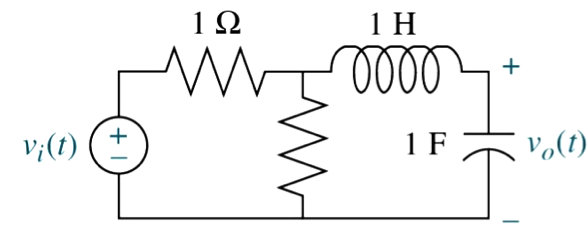
\includegraphics[width=0.5\textwidth]{testfig}
	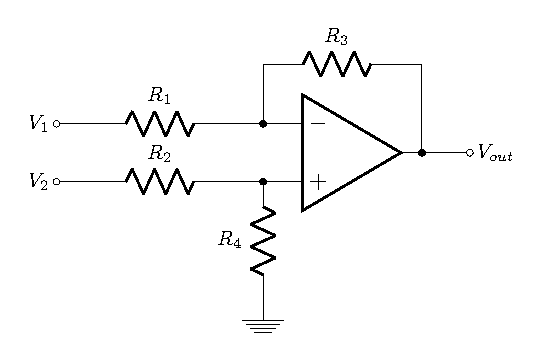
\includegraphics{diffamp}
%	\caption{Differential Amplifier \\ \figurecaption{Penguat Pembeza}}
	\caption{\rajah}
	\label{fig:diffamp4}
\end{figure}

\captionsetup[table]{labelsep=colon, labelfont=bf} 	% no bold table
\renewcommand{\arraystretch}{1.2}	% to make better spacing between rows
% Table generated by Excel2LaTeX from sheet 'Sheet1'
\begin{table}[H]
	\centering
	\caption{Freq. vs Magnitude \\ \tablecaption[\jadualbf]{Frekuensi vs Magnitud}}
	%	\caption{\jadual}	% no caption
	%	\begin{tabularx}{220pt}{c c}
	\begin{tabular}{|c|c|}
		%\toprule
		\hline
		%\toprule[1.5pt]
		\multicolumn{1}{|l|}{\textbf{Frequency}} & \multicolumn{1}{l|}{\textbf{Impedance (Magnitude) ($\Omega$)}} \\
		%\midrule
		\hline
		5 Hz  & 20,000 \\
		10 Hz & 19,998 \\
		\vdots     & \vdots \\
		40 kHz & 602 \\
		50 kHz & 600 \\
		100 kHz & 600 \\
		\hline
		%\bottomrule
		%\bottomrule[1.5pt]
	\end{tabular}
	%		\end{tabularx}%
	\label{table:freqmag3}%
\end{table}%

\paperend

\end{document}